\documentclass[12pt,a4paper]{article}
\usepackage{graphicx, booktabs, siunitx, amsmath, geometry, float}
\usepackage{subcaption}
\geometry{margin=2.5cm}
\title{M4: Digital Logic Circuits}
\author{Gregorio Jaca U8L9B9 gregorio.jaca@gmail.com , \\ Peter Tallosy K14WR1 peter@tallosy.hu }
\date{2025.11.06}

\begin{document}
\maketitle

\begin{abstract}
In this laboratory exercise, we investigated digital logic circuits. We analyzed a black-box on an unknown integrated circuit, which we identified as an SN74LS00 NAND gate, by determining its truth table and measuring its output voltage levels. We also characterized its behavior as an inverter and measured its signal propagation delays at different frequencies. Additionally, we assembled and observed the behavior of a binary counter, describing the relationship between its outputs and the input clock signal, recording its truth table, and displaying it with a seven-segment display.
\end{abstract}

\section{Introduction}
Digital electronics are the foundation of modern computing and control systems. The basic building blocks of these systems are logic gates, which perform logical operations on binary inputs. Sequential circuits, such as counters, are also fundamental, allowing for time-dependent operations and storage of information. The purpose of this measurement was to gain practical experience with both of these components. Our tasks involved identifying an unknown logic gate through its behavior and truth table, and examining the operation of a multi-bit counter and building it.

\section{Results}

\subsection{Black Box Analysis}

\subsubsection{Characterization}

We were given an SN74LS00 integrated circuit and tasked with its characterization. A Vcc of \SI{5}{\volt} was applied to pin 14, with pin 7 connected to ground. We treated the IC as a black box, using pins 1 and 2 as inputs (A and B) and pin 3 as the output (F). We applied all possible combinations of logical low (\SI{0}{\volt}) and logical high (\SI{5}{\volt}) to the inputs and measured the corresponding output voltage. The results are summarized in Table \ref{tab:truth_table_nand}. The measured high output voltage was approximately \SI{4}{\volt}, and the low output voltage was \SI{0.17}{\volt}.

\begin{table}[H]
    \centering
    \caption{Measured truth table for the two-input logic gate.}
    \begin{tabular}{cc|c}
        \toprule
        \multicolumn{2}{c|}{Inputs} & Output \\
        A & B & F \\
        \midrule
        0 & 0 & 1 \\
        1 & 0 & 1 \\
        0 & 1 & 1 \\
        1 & 1 & 0 \\
        \bottomrule
    \end{tabular}
    \label{tab:truth_table_nand}
\end{table}

The observed behavior, where the output is low only when both inputs are high, is a NAND gate. We then veryfied this by checking the SN74LS00 data sheet, where we confirmed that it is a bipolar NAND gate.

\subsubsection{Inverter Configuration}
By connecting inputs A and B together, we created a single-input gate. We tested its behavior, and the results are shown in Table \ref{tab:truth_table_not}.

\begin{table}[H]
    \centering
    \caption{Measured truth table for the single-input configuration.}
    \begin{tabular}{c|c}
        \toprule
        Input & Output \\
        A & F \\
        \midrule
        0 & 1 \\
        1 & 0 \\
        \bottomrule
    \end{tabular}
    \label{tab:truth_table_not}
\end{table}

This configuration inverts the input signal, functioning as a NOT gate. The switching thresholds were observed to be between the high state of \SI{4}{\volt} and the low state of \SI{0.17}{\volt}. There is hysterisis in the switching which is benefitial for a comparator to be less noise suceptible. Other gates can be created from combinations of NAND gates.

\subsubsection{Timing Analysis}
We applied a square wave signal to the input of the inverter configuration to measure the propagation delay. The output signal's rise and fall times were observed relative to the input signal. Figure \ref{fig:timing} shows the oscilloscope readings for input frequencies of \SI{1}{\hertz} and \SI{1}{\kilo\hertz}. We measured the rise time and fall time, which are the time it takes for a signal transition to go from 10\% to 90\% of its value after the switch and we report the values \footnote{For the 1Hz signal we only measured one switch, so we could not report the error, while for the 1kHz signal we measured 7 switches, allowing us to report more accurate results.}. 

% At \SI{1}{\hertz}, the fall time was \SI{10.2}{\micro\second} and the rise time was \SI{10}{\micro\second}. At \SI{1}{\kilo\hertz}, the fall time was \SI{10.2}{\micro\second} and the rise time was \SI{10}{\micro\second} .

\begin{table}[H]
    \centering
    \caption{Rise and fall times at \SI{1}{\hertz}}
    \begin{tabular}{lcc}
        \toprule
        Channel & Mean Time (\si{\micro\second}) \\
        \midrule
        CH1 (fall) & 1640.20 \\
        CH2 (rise) & 1640.00 \\
        \bottomrule
    \end{tabular}
\end{table}

\begin{table}[H]
    \centering
    \caption{Rise and fall times at \SI{1}{\kilo\hertz}}
    \begin{tabular}{lcc}
        \toprule
        Channel & Mean Time (\si{\micro\second}) & Std. Dev. (\si{\micro\second}) \\
        \midrule
        CH1 (rise) & 500.00 & 0.00003 \\
        CH1 (fall) & 500.00 & 0.00005 \\
        CH2 (rise) & 500.00 & 0.00005 \\
        CH2 (fall) & 500.00 & 0.00003 \\
        \bottomrule
    \end{tabular}
\end{table}

% At \SI{1}{\kilo\hertz}, the measured delay for a rising edge at the output was approximately \SI{500000}{ns} (\SI{0.5}{ms}), and the delay for a falling edge was also approximately \SI{500000}{ns}. This corresponds to half the period of the \SI{1}{\kilo\hertz} signal, indicating the inversion of the signal.

\begin{figure}[H]
    \centering
    \begin{subfigure}[b]{0.48\linewidth}
        \centering
        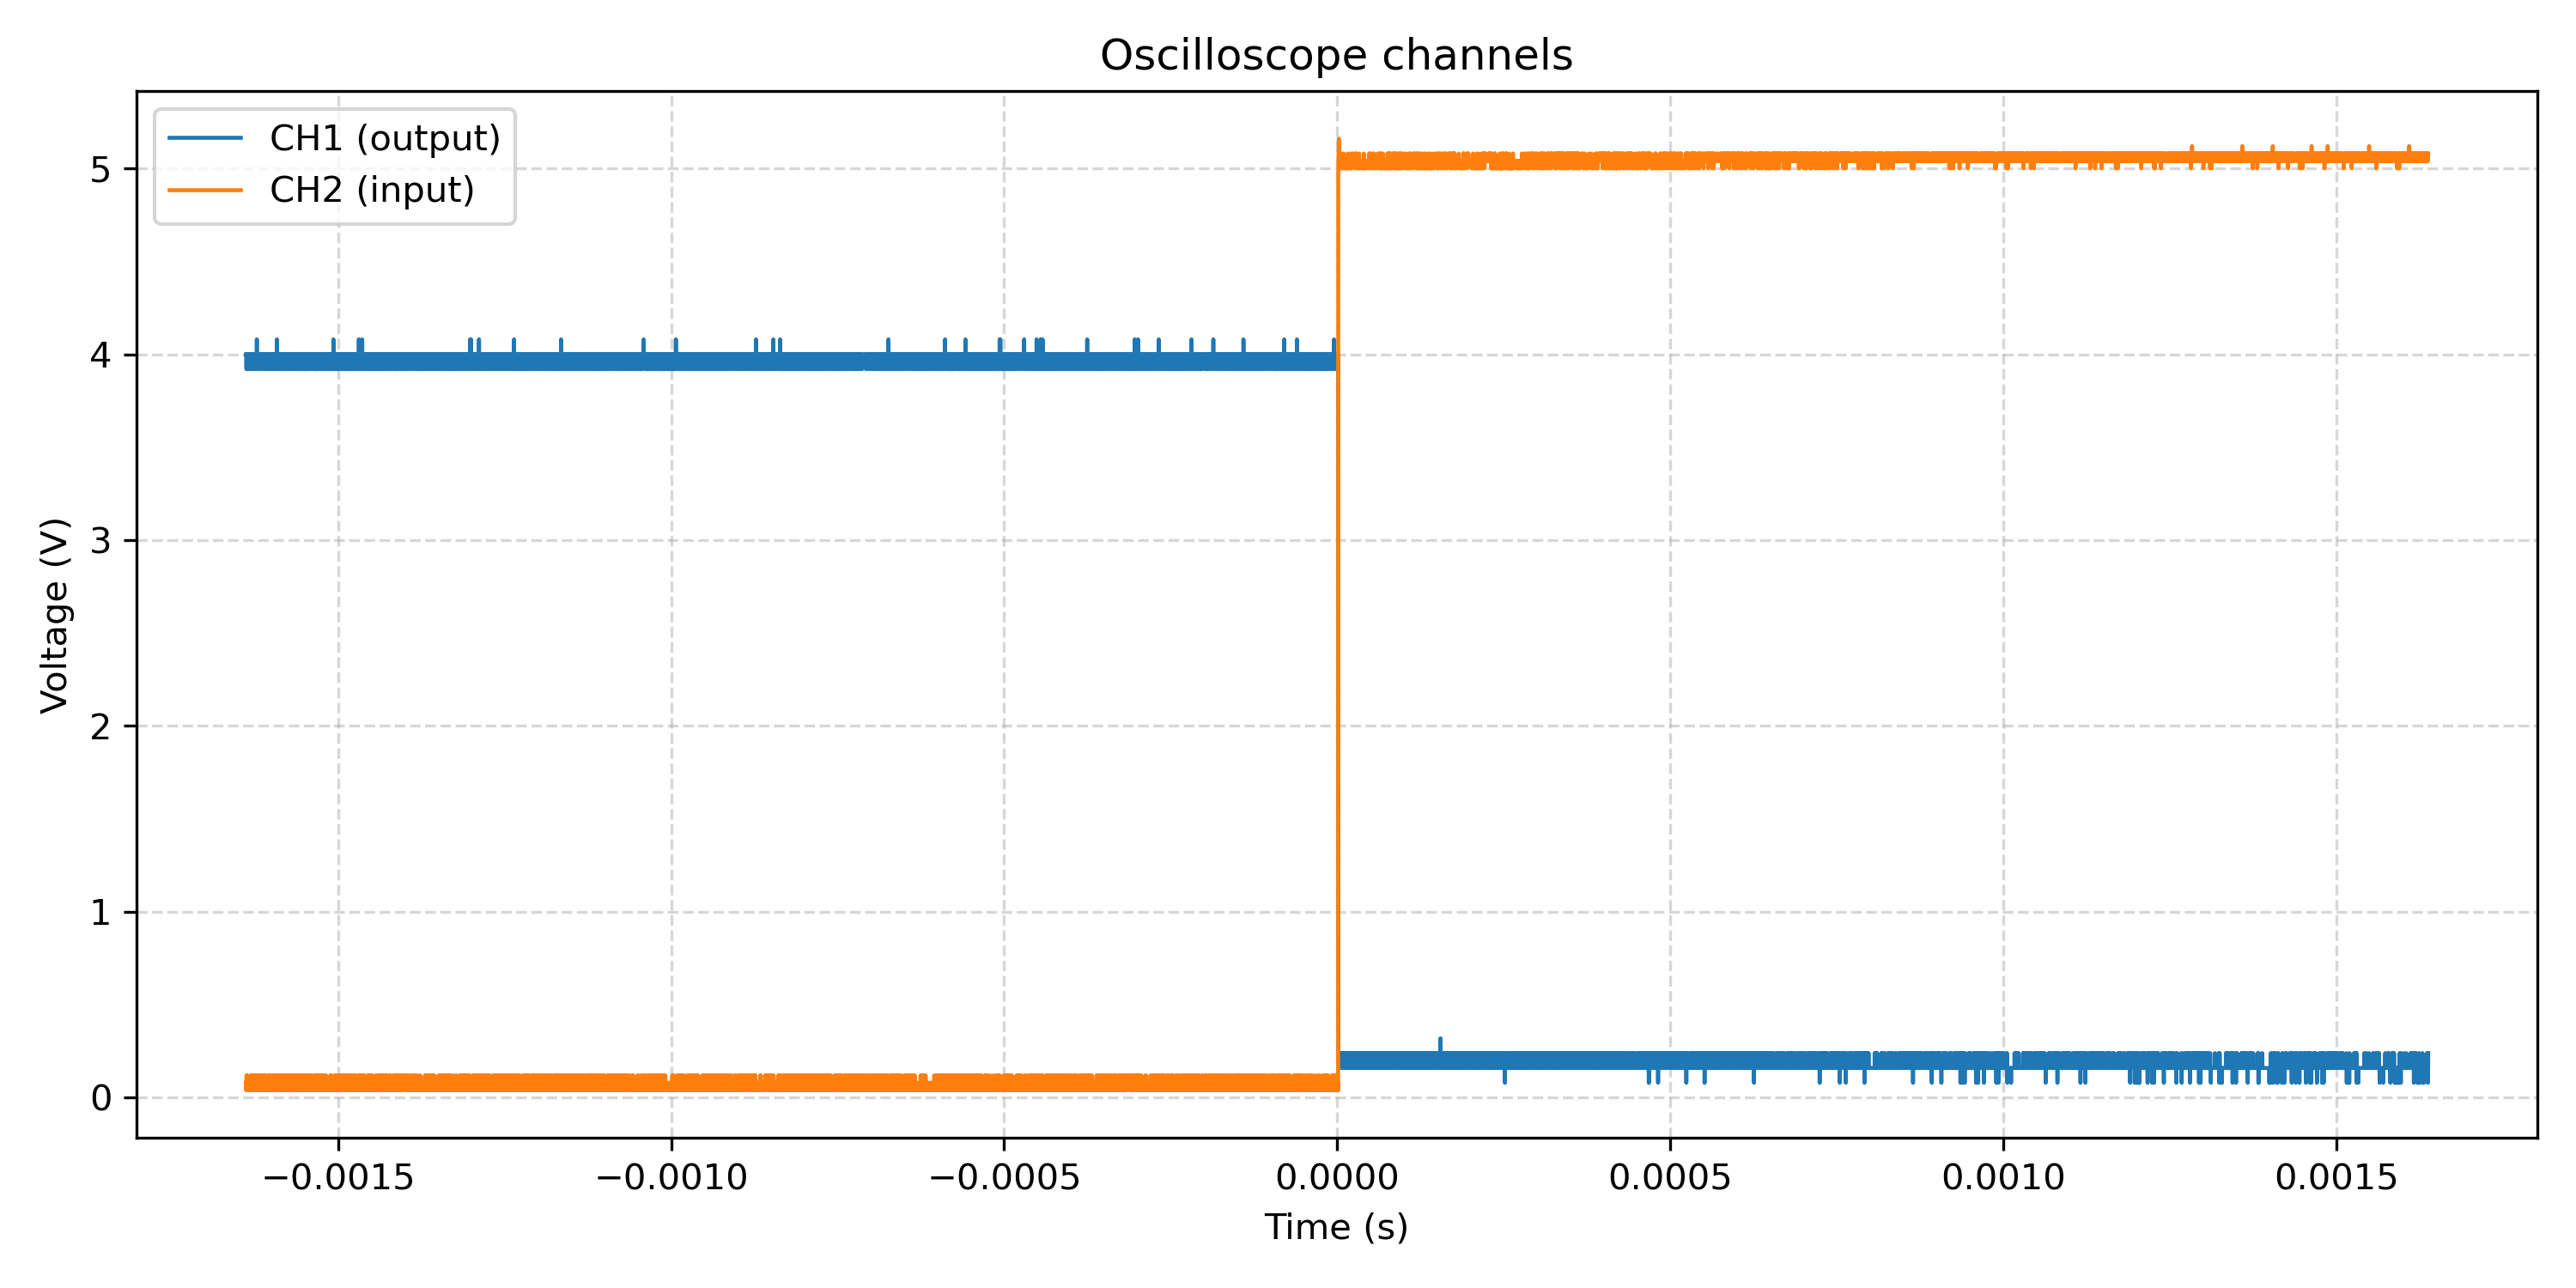
\includegraphics[width=\linewidth]{1Hz.png}
        \caption{Input (top) and output (bottom) signals at \SI{1}{\hertz}.}
    \end{subfigure}\hfill
    \begin{subfigure}[b]{0.48\linewidth}
        \centering
        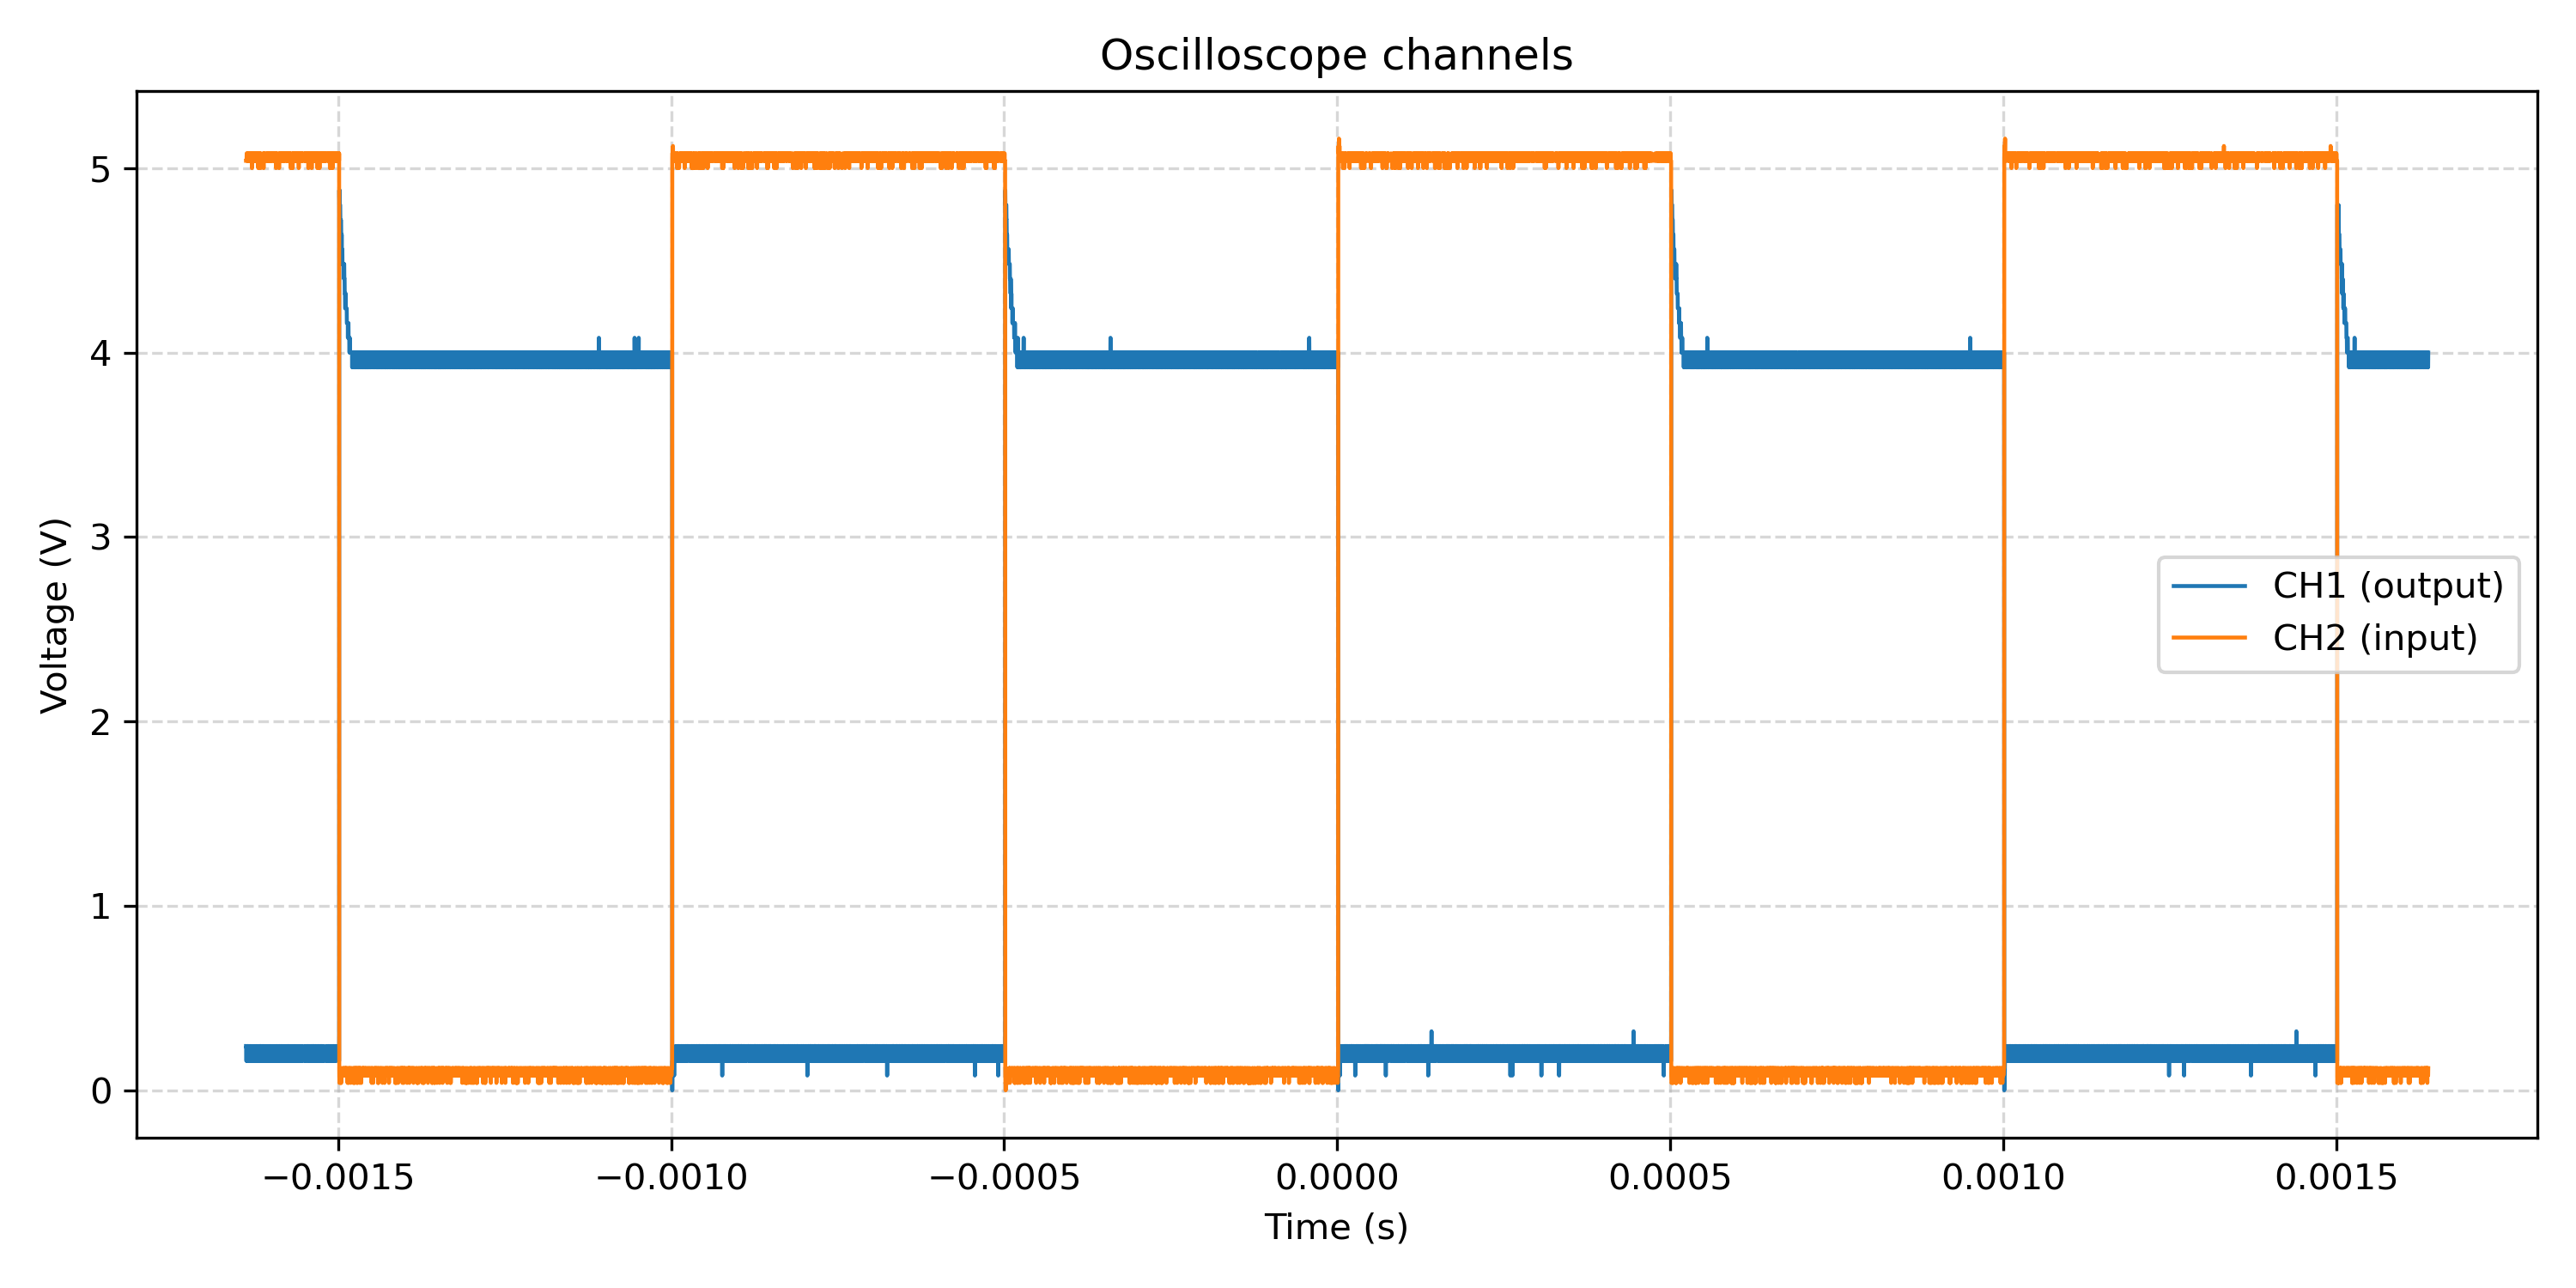
\includegraphics[width=\linewidth]{1kHz.png}
        \caption{Input (top) and output (bottom) signals at \SI{1}{\kilo\hertz}.}
    \end{subfigure}
    \caption{Oscilloscope view of the inverter's input and output signals at different frequencies.}
    \label{fig:timing}
\end{figure}

\subsection{BCD Counter}

\subsubsection{Counter Operation}
We assembled a circuit with a binary counter. We observed its output behavior when a 1Hz square clock signal was applied by connecting each bit to a LED as can be seen in Fig. \ref{fig:LED}. There was a change in the state every 1 second because that is the time period of the 1Hz clock signal. The truth table for the first three bits of the counter is shown in Table \ref{tab:counter_truth_table_4bit}.

\begin{table}[H]
    \centering
    \caption{Truth table for a 4-bit binary counter.}
    \begin{tabular}{cccccc}
        \toprule
        count & Q3 & Q2 & Q1 & Q0 \\
        \midrule
         0 & 0 & 0 & 0 & 0 \\
         1 & 0 & 0 & 0 & 1 \\
         2 & 0 & 0 & 1 & 0 \\
         3 & 0 & 0 & 1 & 1 \\
         4 & 0 & 1 & 0 & 0 \\
         5 & 0 & 1 & 0 & 1 \\
         6 & 0 & 1 & 1 & 0 \\
         7 & 0 & 1 & 1 & 1 \\
         8 & 1 & 0 & 0 & 0 \\
         9 & 1 & 0 & 0 & 1 \\
        10 & 1 & 0 & 1 & 0 \\
        11 & 1 & 0 & 1 & 1 \\
        12 & 1 & 1 & 0 & 0 \\
        13 & 1 & 1 & 0 & 1 \\
        14 & 1 & 1 & 1 & 0 \\
        15 & 1 & 1 & 1 & 1 \\
        \bottomrule
    \end{tabular}
    \label{tab:counter_truth_table_4bit}
\end{table}


We observed that the least significant bit (LSB) toggled its state with every clock pulse. The second bit toggled at half the frequency of the LSB (every two clock pulses), and the third bit toggled at a quarter of the frequency (every four clock pulses). 
% This hierarchical division of frequency is the defining characteristic of a binary ripple counter.
% !!!!!!!!!!!

\begin{figure}[H]
    \centering
    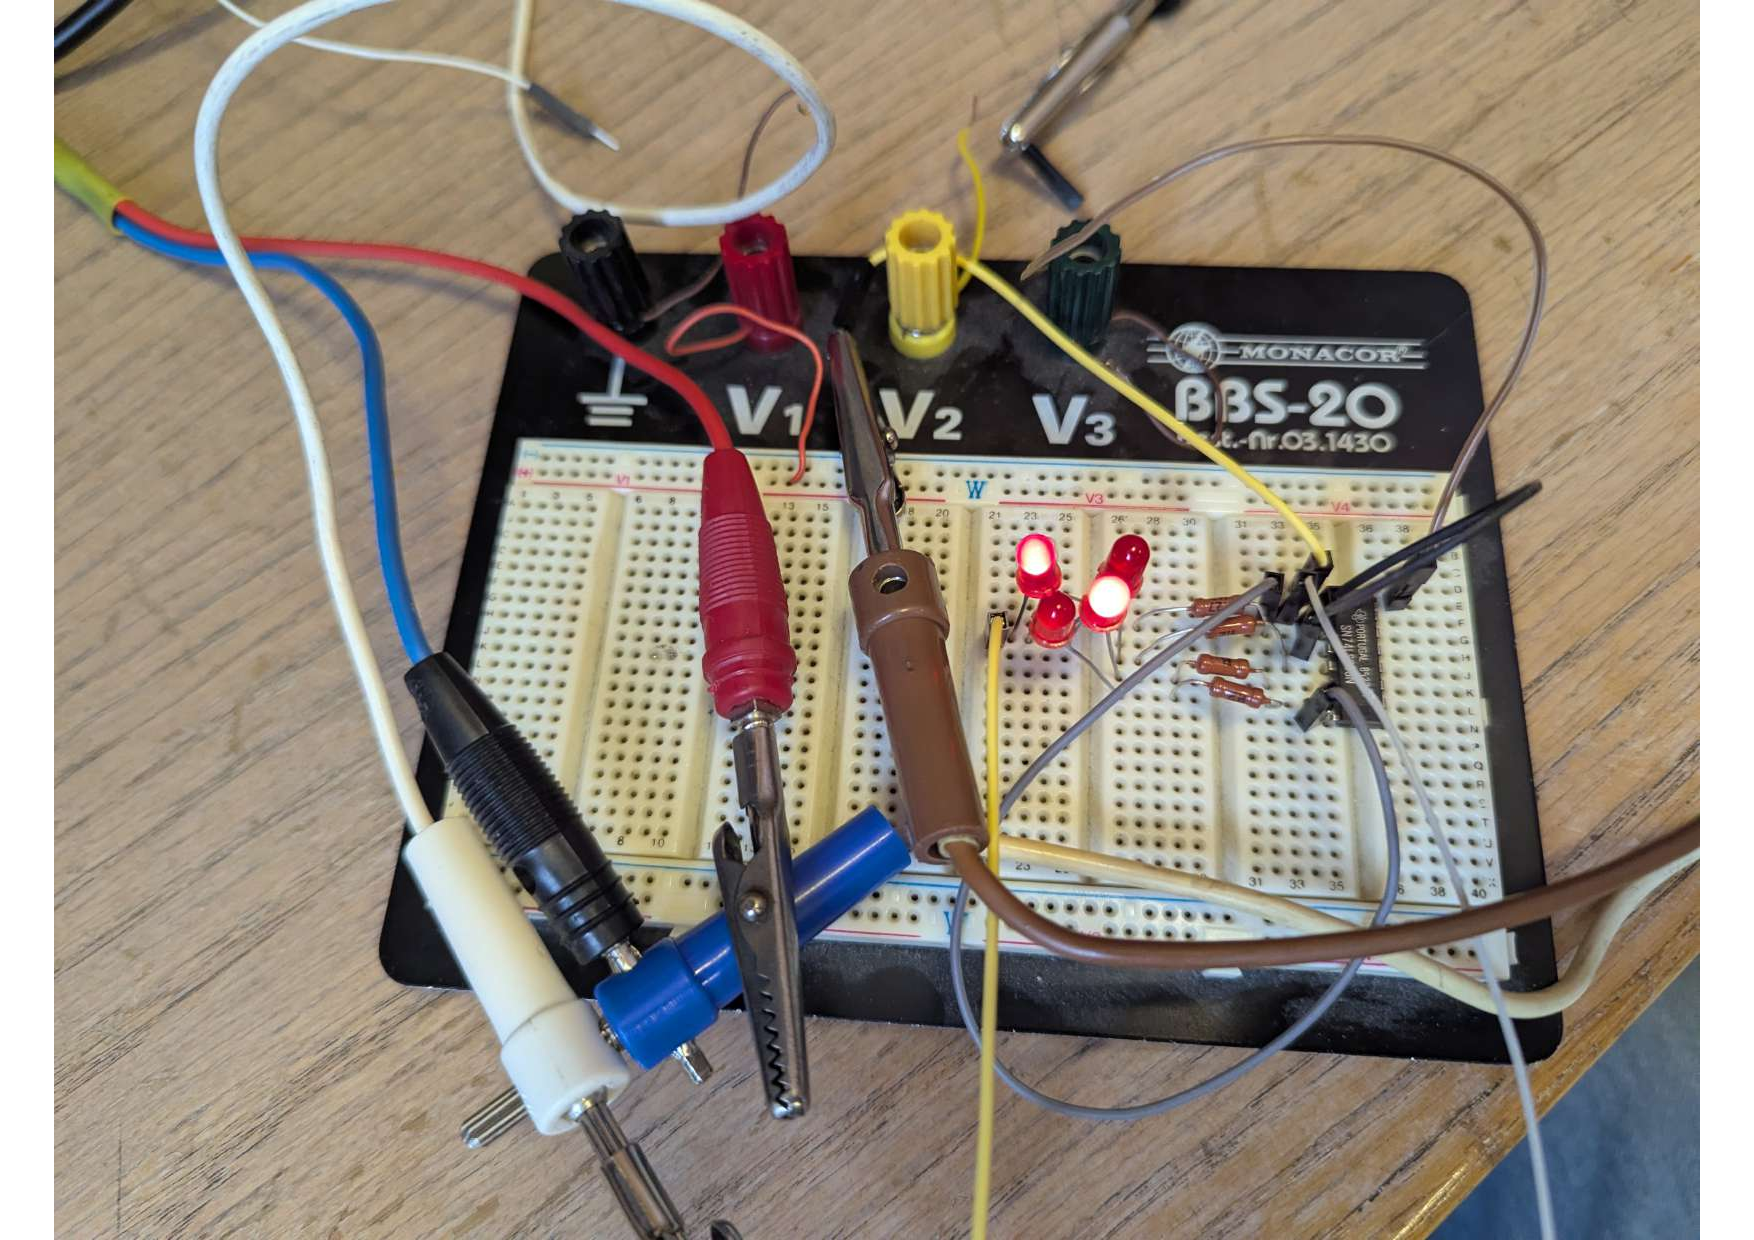
\includegraphics[width=0.7\linewidth]{truth_table.pdf}
    \caption{4-bit binary counter with the LEDs visualizing each bit (the most significant digit is at the front). The configuration showed corresponds to the (0,1,0,1) state, which corresponds to the number 5.}
    \label{fig:LED}
\end{figure}

\subsubsection{Decoder and Display}
We extended the circuit with an SN7447 decoder and a 7-segment display, which allowed us to display the numbers is base 10 format.

\begin{figure}[H]
    \centering
    \begin{subfigure}[b]{0.48\linewidth}
        \centering
        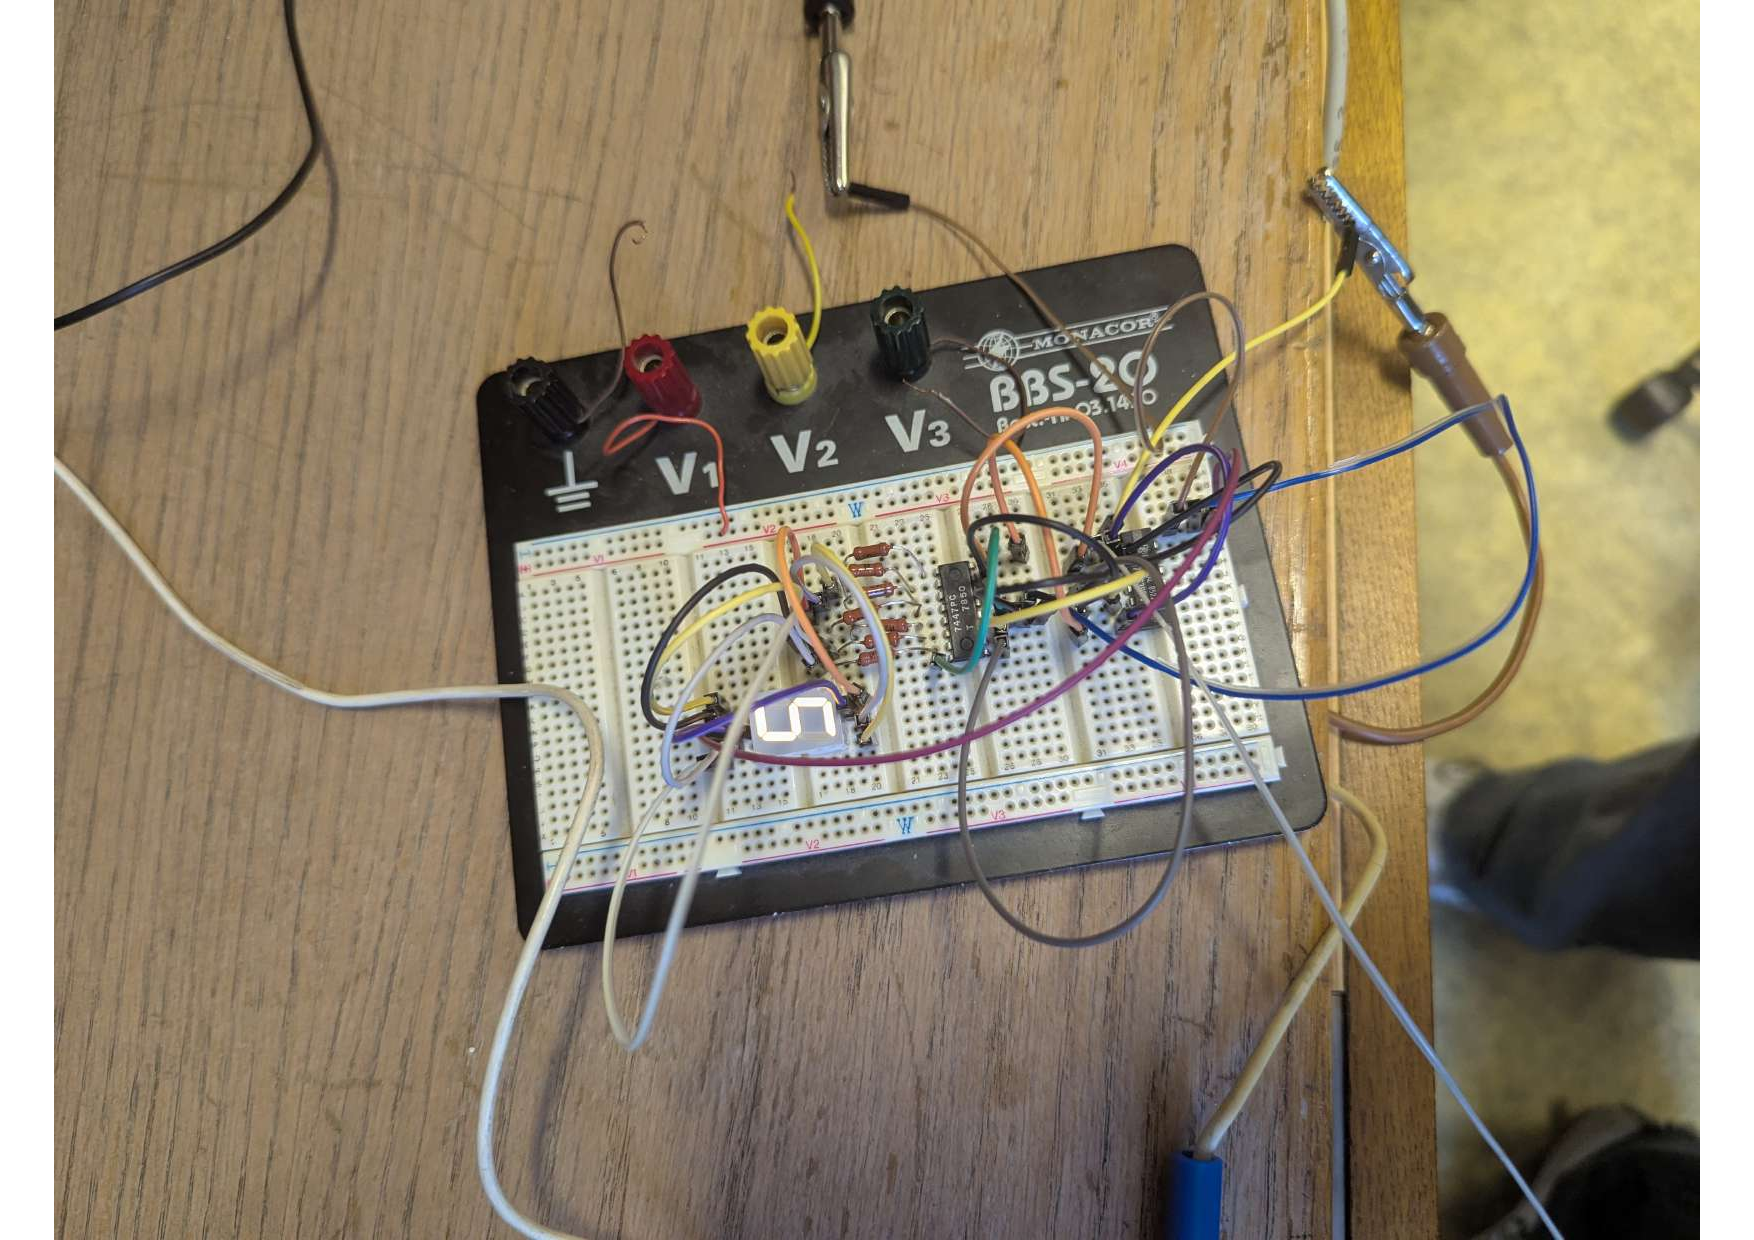
\includegraphics[width=\linewidth]{5.pdf}
        % \caption{Counter displaying.}
    \end{subfigure}\hfill
    \begin{subfigure}[b]{0.48\linewidth}
        \centering
        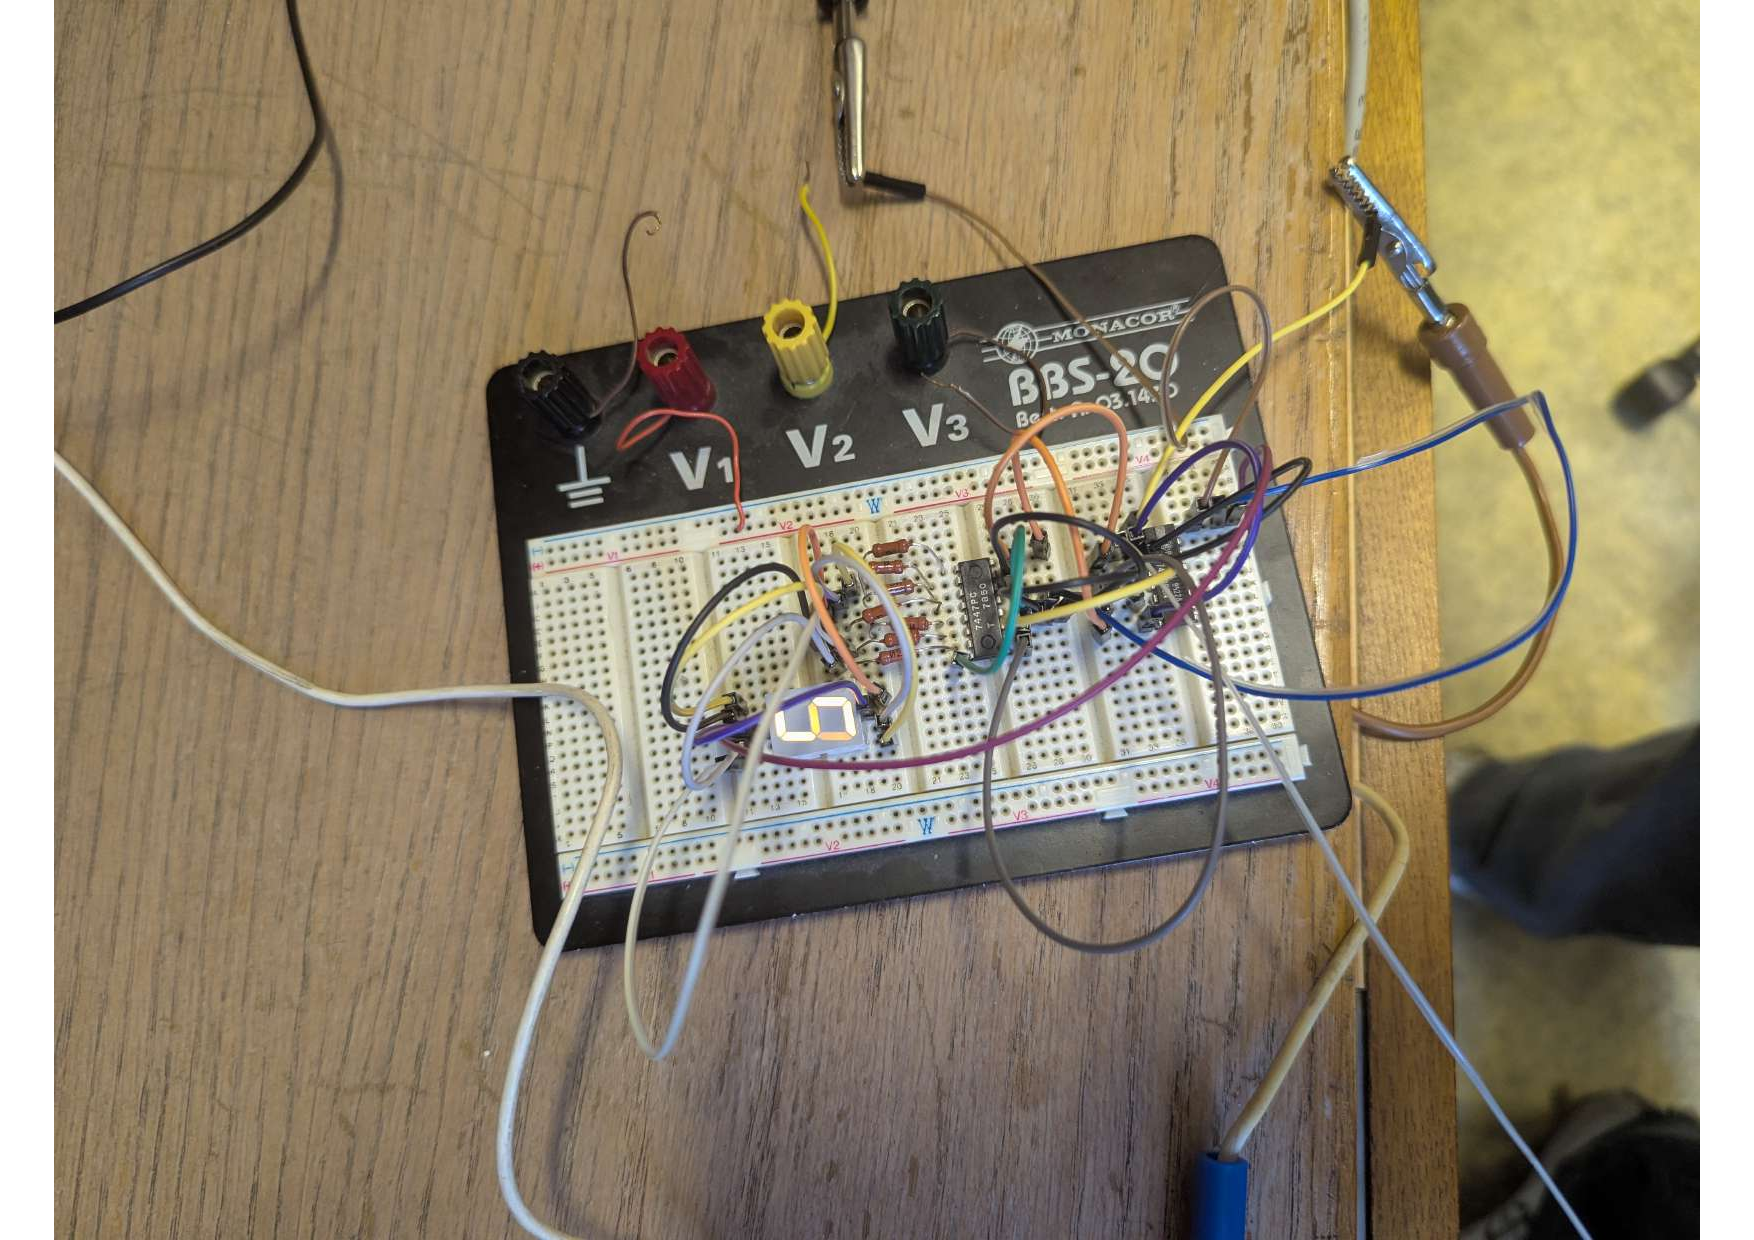
\includegraphics[width=\linewidth]{6.pdf}   
        % \caption{.}
    \end{subfigure}
    \caption{Counter showing a 5 (left) and a 6 (right). }
    \label{fig:photos56}
\end{figure}


\subsubsection{Reset at 6}

In table \ref{tab:counter_truth_table_4bit} we saw how the number is represented as a (0,1,1,0), and this is the first element in the series where the two middle digits (Q1 and Q2) are "1". Because we want to reset at the number 6, we need an AND gate whose input is connected to Q1 and Q2 and the output connected to the counter's reset. We have a NAND gate and we saw how to buold a NOT gate, so we can easily build an AND gate by connecting them in this order NAND -> NOT, obtainning the required circuit element. We started this process, but due to time constraints, were unable to finalize. The only thing we are unsure of is: do we want to reset immediatly after getting the "6" or do we want to display it for the duration of the counter's period (in the case of the 1Hz driving, then 1 second), because in the latter case, we would need to reset at the end of the digit 6, which would require us to trigger the reset when the digit 7 is outputted. In that case, because 7 is represented as (0,1,1,1) we need two AND gates to trigger the reset (for example, one connected to Q0 and Q1, and the other connected to Q2 and the output of the previous AND gate). The SN7447 master reset is async so, we expect an immediate reset. If it were sync, then it would reset at the next clock signal (displaying the digit for extra time during the clock's period).

\subsection{Power rating of the series resistor}

Using: $V_{\text{high}} = 5\ \text{V}$, $V_{\text{LED}} = 1.8\ \text{V}$, $I_{\text{LED}} = 10\ \text{mA}$, $R = 270\ \Omega$.

The voltage across the resistor is:
\[
V_R = V_{\text{high}} - V_{\text{LED}} = 5 V - 1.8 V = 3.2\ \text{V}.
\]

The current through the resistor (and LED) is designed to be approximately $I = 10\ \text{mA} = 0.01\ \text{A}$. Then, the power dissipated in the resistor:
\[
P = I^2 R = (0.01)^2 \times 270 = 0.027\ \text{W} \quad (27\ \text{mW}).
\]

A standard rated 1/8 W (0.125 W) resistor is more than sufficient, providing a safety margin.

\section{Conclusion}
In this measurement, we successfully characterized an SN74LS00 IC, confirming its function as a NAND gate and demonstrating its use as a NOT gate. We measured its static voltage levels for high and low states and observed its dynamic behavior, noting the inversion of the input signal. Our attempt to build and test a BCD counter with a 7-segment display was partially successful; we were able to observe the fundamental counting behavior, but the full circuit with the display did not work. This exercise provided hands-on experience with the basic principles of digital logic circuits.

\section{Equipment Used}
\begin{itemize}
    % \item Op-Amps: \textmu A741, TL071
    % \item Transistors: BC182
    \item BCD counter: 7447PC (TTL BCD-to-7-segment decoder/driver)
    \item Black-Box (NAND gate): SN74LS00
    \item DC Power Supply: Siglent SPD3303C
    % \item Digital Multimeter: Siglent SDM 3045X and UNI-T UT334+
    \item Function Generator: RIGOL DG811 SiFi II 20MHz AWG
    \item Oscilloscope: SIGLENT SDS 1072CML Digital Oscilloscope
    \item Resistors and Capacitors of various values. Breadboard and Wires.
\end{itemize}

\end{document}
